%
% einleitung.tex -- Beispiel-File für die Einleitung
%
% (c) 2020 Prof Dr Andreas Müller, Hochschule Rapperswil
%
% !TEX root = ../../buch.tex
% !TEX encoding = UTF-8
%
% erste Maxwellgleichung ohne Quelle

\tikzset{>=latex} % for LaTeX arrow head
\usetikzlibrary {arrows.meta}
\pgfplotsset{compat=1.13}
\usetikzlibrary{decorations.markings,intersections,calc}
\usetikzlibrary{angles,quotes} % for pic (angle labels)
\colorlet{Ecol}{green!90!black}
\colorlet{EcolFL}{green!80!black}
\colorlet{Bcol}{blue!90!black}
\tikzstyle{EcolEP}=[blue!80!white]
\colorlet{veccol}{green!45!black}
\tikzstyle{charge+}=[very thin,top color=red!50,bottom color=red!90!black,shading angle=20]
\tikzstyle{charge-}=[very thin,top color=blue!50,bottom color=blue!80,shading angle=20]
\tikzstyle{charge_small} = [very thin,top color=red!50,bottom color=red!90,shading angle=20]
\tikzstyle{vector}=[->,thick,veccol]
\tikzset{EFieldLineArrow/.style={EcolFL,decoration={markings,mark=at position #1 with {\arrow{latex}}},
		postaction={decorate}},
	EFieldLineArrow/.default=0.5}


\section{Elektrostatik\label{maxwell:section:elekktrostatik}}
\rhead{Elektrostatik}
Die Elektrostatik ist ein Spezialfall der Elektrodynamik, bei dem statische, das heisst zeitlich nicht veränderliche Felder betrachtet werden.
Dies setzt voraus, dass
\begin{equation}
	\frac{\partial f}{\partial t}
	=
	0
	\label{maxwell:section:definition_statik}
\end{equation}
für alle Funktionen gilt, welche wir in diesem Abschnitt betrachten.
Daraus folgt, dass uns nur ruhende Ladungen interessieren.
Dies hat zur Folge, dass keine Stromdichten existieren können, weil
\begin{equation}
	\varrho\,\vec{v}
	=
	\varrho\, \underbrace{\frac{\partial \vec{x}}{\partial t}}_{=0}
	=
	\vec{\jmath}
	=
	0.
\end{equation}
Im späteren Abschnitt \ref{maxwell:magnetostatik} der Magnetostatik wird klar, dass aus diesem Grund in der Elektrostatik keine magnetische Flussdichte existieren kann.
 
Das Ziel ist nun, das elektrische Feld im Zusammenspiel mit ruhenden Ladungen zu beschreiben.
Dafür werden wir in den folgenden Abschnitten die nötigen Begriffe definieren und genauer erklären.

\subsubsection{Elektrisches Potentialfeld}
Das elektrische Potentialfeld
\(
\varphi:\mathbb{R}^3
\rightarrow
\mathbb{R}
\)
ist als
\begin{equation}
	\varphi(x,y,z)
	=
	\frac{W_{\text{pot}}(x,y,z)}{q}
	\label{maxwell:section:definition_elektrischespotentialfeld}
\end{equation}
definiert.
In Worten gefasst kann man sagen, dass das elektrische Potential eine auf die Ladung normierte potentielle Energie darstellt.
Somit kann die linke Abbildung in \ref{maxwell:skalarGrad} als ein Feld, das proportional zur potentiellen Energie ist, angeschaut werden.
Des weiteren steht die elektrische Spannung eng in Verbindung mit dem elektrischen Potential.
Die Spannung $U$ zwischen zwei Punkten $a$ und $b$ wird definiert als
\(
U_{ab}
=
\varphi_a - \varphi_b.
\)
% not sure about this
Das heisst die Spannung ist der Potentialunterschied zwischen zwei Punkten.

\subsubsection{Elektrisches Feld}
Das elektrische Feld
\(
\vec{E}:\mathbb{R}^3 \rightarrow \mathbb{R}^3
\)
wird in der Elektrostatik definiert als
\begin{equation}
	\vec{E}
	=
	- \nabla\varphi.
	\label{maxwell:section:definition_statisch_elektrischesFeld}
\end{equation}
Diese Definition besagt, dass das elektrische Feld ein statisches Gradientenfeld ist.
Dieses Feld kann man anhand der Kraftwirkung an sogenannten Probeladungen $q$ messen, da
\[
\vec{E}
=
\frac{\vec{F}}{q}
\]
ist.
Somit sind die Vektoren in Abbildung \ref{maxwell:section:E-Feld_punktladung} Kraftvektoren, welche normiert sind auf die Ladung $q$.
%E-Field of point charge
\begin{figure}
	\centering
	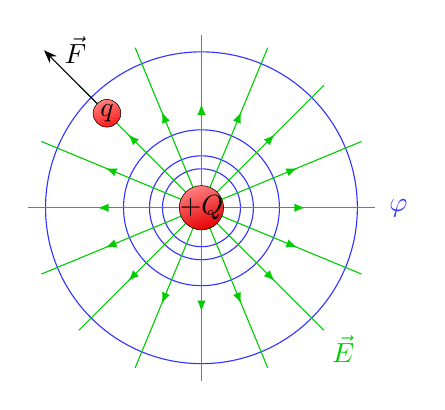
\begin{tikzpicture}
		\def\R{2.2}
		\def\NE{16}
		\def\NV{4}
		\contourlength{1.6pt}
		
		\foreach \i [evaluate={\r=0.9*\R/\i;}] in {1,...,\NV}{
			\draw[EcolEP] (0,0) circle (\r);
		}
		
		\foreach \i [evaluate={\angle=(\i-1)*360/\NE;}] in {1,...,\NE}{
			\draw[EFieldLineArrow={0.6}] (0,0) -- (\angle:\R);
		}
		\draw[charge+] (0,0) circle (8pt) node[black,scale=1] {$+Q$};
		%\draw[FFieldLineArrow={0.6}] (-1,1) -- (-2,2);
		\draw[-{Stealth[black]}] (-1.2,1.2) -- (-2,2) node at (-1.6, 2) {$\vec{F}$};
		\draw[charge_small] (-1.2,1.2) circle (5pt) node[black,scale=1] {$q$};
		\node[EcolFL,scale=1] at (1.8,-1.8) {$\vec{E}$};
		\node[EcolEP,scale=1] at (2.5,0) {$\varphi$};
	\end{tikzpicture}
	\caption{Elektrisches Feld (grün) einer positiven Punktladung $+Q$ und Äquipotentiallinien (blau) der selben positiven Punktladung $+Q$}
	\label{maxwell:section:E-Feld_punktladung}
\end{figure}


\subsubsection{Energiedichte im elektrischen Feld}
Das elektrische Feld beinhaltet eine Energie und somit auch eine Energiedichte.
Diese Energiedichte ist definiert als
\begin{equation}
w_{\text{e}}
=
\frac{1}{2}\,\varepsilon\,\vec{E}\,^2,
\label{maxwell:section:definiton_energiedichte_elektrischesFeld}
\end{equation}
wobei $\varepsilon$ die Permittivität ist.
Die Permittivität
\(
\varepsilon
=
\varepsilon_r\,\varepsilon_0
\)
ist ein Mass dafür, wie gut sich ein Material polarisieren lässt und ist das Produkt der relativen Permittivität $\varepsilon_r$ und der Permittivität vom Vakuum $\varepsilon_0$.
Die relative Permittivität ist eine materialabhängige Grösse und hat im Vakuum den skalaren Wert $1$.
Die Permittivität des Vakuums in SI-Einheiten
\[
\varepsilon_0
=
8.854 \cdot 10^{-12}\,\frac{\text{C$^2$}}{\text{Nm$^2$}}
\]
ist die elektrische Feldkonstante.

\subsection{Laplace-Gleichung
	\label{maxwell:section:elektrostatik_ohne_quelle}}
Man stelle sich nun einen ladungsfreien, luftleeren, drei dimensionalen Raum $V\subset\mathbb{R}^3$
vor, indem ein elektrisches Potentialfeld $\varphi(x,y,z)$ existiert.
Für diesen Raum möchten wir mittels der Variationsrechnung eine partielle Differentialgleichung entwickeln, die beschreibt, wie sich das Potentialfeld und somit auch das elektrische Feld verhält. 

\subsubsection{Ansatz}
Damit wir eine Gleichung erhalten, die das Verhalten des elektrischen Potentialfeldes beschreibt, muss ganz allgemein die Energie im System minimiert werden. 
In diesem Fall ist die Energie im System
\[
W_{\text{e}}
=
\iiint_V w_e\, dV.
\]
Dieses Integral gilt es zu minimieren, was die Grundlage für unser Variationsproblem darstellt.
Die in \eqref{maxwell:section:definiton_energiedichte_elektrischesFeld} definierte Energiedichte ist im Vakuum
\[
w_{\text{e}}
=
\frac{1}{2}\,\varepsilon_0\,\vec{E}\,^2.
\]
Diese Gleichung können wir nun mittels Definition \eqref{maxwell:section:definition_statisch_elektrischesFeld} mit dem elektrischen Potentialfeld ausdrücken.
Folglich ist
\begin{align}
\renewcommand{\arraystretch}{1.9}
w_{\text{e}}
&=
\frac{1}{2}\,\varepsilon_0\left(-\nabla\varphi\right)^2
\\
w_{\text{e}}
&=
\frac{1}{2}\,\varepsilon_0
\begin{pmatrix}
\displaystyle
-\varphi_x\\
\displaystyle
-\varphi_y\\
\displaystyle
-\varphi_z
\end{pmatrix}
\cdot
\begin{pmatrix}
\displaystyle
-\varphi_x\\
\displaystyle
-\varphi_y\\
\displaystyle
-\varphi_z
\end{pmatrix}
=
\frac{1}{2}\,\varepsilon_0\left(\varphi_x^2 + \varphi_y^2 + \varphi_z^2\right).
\label{maxwell:section:energiedichte}
\end{align}
Dies können wir in das zu minimerende Integral einsetzen und bekommen
\begin{equation}
	W_{\text{e}}
	=
	\iiint_V \frac{1}{2}\,\varepsilon_0\left(\varphi_x^2 + \varphi_y^2 + \varphi_z^2\right)\, dV.
	\label{maxwell:section:energieintegral_quellenfrei}
\end{equation}
Aus dieser Gleichung können wir entnehmen, dass unsere Lagrange-Funktion
\begin{equation}
	L(x,y,z,\varphi,\varphi_x,\varphi_y,\varphi_z)
	=
	\frac{1}{2}\,\varepsilon_0\left(\varphi_x^2 + \varphi_y^2 + \varphi_z^2\right)
	\label{maxwell:section:lagrangefunktion_quellenfrei}
\end{equation}
ist.
Somit haben wir unsere Lagrange-Funktion gefunden, die wir in einem nächsten Schritt in die Euler-Ostrogradski-Differentialgleichung einsetzen können.

\subsubsection{Einsetzen in die Euler-Ostrogradski-Differentialgleichung}
Nun gilt es die in \eqref{maxwell:section:lagrangefunktion_quellenfrei} gefundene Gleichung in die Euler-Ostrogradski-Differentialgleichung \eqref{buch:felder:ostrogradski:eqn:euler-ostrogradski} einzusetzen.
Nach Einsetzen wird die Differentialgleichung zu
\begin{align*}
\frac{1}{2}\,\varepsilon_0\,\biggl(\underbrace{\frac{\partial}{\partial\varphi}\left(\varphi_x^2 + \varphi_y^2 + \varphi_z^2\right)}_{\displaystyle=0} &- \frac{\partial}{\partial x}\frac{\partial}{\partial \varphi_x}\left(\varphi_x^2 + \varphi_y^2 + \varphi_z^2\right)\\
&- \frac{\partial}{\partial y}\frac{\partial}{\partial \varphi_y}\left(\varphi_x^2 + \varphi_y^2 + \varphi_z^2\right) - 
\frac{\partial}{\partial z}\frac{\partial}{\partial \varphi_z}\left(\varphi_x^2 + \varphi_y^2 + \varphi_z^2\right)\biggr)
=
0.
\end{align*}
Man sieht, dass die partielle Ableitung nach $\varphi$ verschwindet.
Nachdem wir die partiellen Ableitungen nach $\varphi_x$, $\varphi_y$ und $\varphi_z$ durchgeführt haben, wird die Differentialgleichung zu
\[
\frac{1}{2}\,\varepsilon_0\left(-\frac{\partial}{\partial x}2\varphi_x - \frac{\partial}{\partial y}2\varphi_y - \frac{\partial}{\partial z}2\varphi_z\right)
=
0.
\]
Wenn man nun noch die letzten partiellen Ableitungen durchführt, resultiert
\begin{equation}
	- \varepsilon_0\underbrace{\left(\frac{\partial^2\varphi}{\partial x^2} + \frac{\partial^2\varphi}{\partial y^2} + \frac{\partial^2\varphi}{\partial z^2}\right)}_{\displaystyle=0}
	=
	0.
	\label{maxwell:section:laplace_gleichung_1}
\end{equation}
%TODO:definiton des laplace operators suchen
An dieser Gleichung sieht man, dass die Klammer mit den partiellen Ableitungen gleich null sein muss, da die Permittivität des Vakuums nicht null sein kann.
Zusätzlich wird nun ersichtlich, dass der Klammerterm nach Definition \eqref{buch:felder:fundamentallemma:} mit dem Laplace-Operator angewendet auf das elektrische Potentialfeld $\varphi$ ersetzt werden kann.
Somit wird unsere Schlussdifferentialgleichung zu
\begin{equation}
	\Delta\varphi
	=
	0.
	\label{maxwell:section:laplace_gleichung_2}
\end{equation}
%TODO: Definition Laplace suchen.
Wenn wir nun den Laplace-Operator laut seiner Definition \eqref{buch:felder:fundamentallemma:eqn:laplaceproduktformel} mittels Divergenz und Gradient ausdrücken, erhalten wir die Gleichung
\begin{equation}
\nabla\cdot\underbrace{\nabla\varphi}_{\displaystyle-\vec{E}}
=
0.
\label{maxwell:section:laplace_gleichung_3}
\end{equation}
Dank der statischen Definition des elektrischen Feldes \eqref{maxwell:section:definition_statisch_elektrischesFeld} können wir unsere Schlussdifferentialgleichung auch mit dem elektrischen Feld ausdrücken. Somit erhalten wir, dass
\begin{equation}
	\nabla\cdot\vec{E}
	=
	0
	\label{maxwell:section:e_feld_quellenfrei}
\end{equation}
sein muss. Diese Differentialgleichung besagt, dass das elektrische Feld quellenfrei ist.
Dies bedeutet, dass Felldlinien des elektrischen Feldes an keinem Ort im Raum enstehen oder enden können.
Was wiederum sehr naheliegend ist, da ohne Ladungen im Raum das elektrische Feld quellenfrei sein muss.

%Darf auch weggelassen werden.
\subsubsection{Exkurs zur Laplace-Gleichung}
\label{maxwell:section:laplacegleichung_exkurs}
Ein Potentialfeld, das die Laplace-Gleichung
\[
\Delta\varphi
=
0
\]
erfüllt, führt zu einem Gradientenfeld $\nabla\varphi$, das rotationsfrei und quellenfrei ist.
Diese Gleichung findet nicht nur Anwendungen in der Elektrostatik, sondern auch in stationärer Fluiddynamik und stationärer Wärmeleitung.






